前面的章節中已經注意到,高效的程序需要充分利用可用的硬件資源,而不是把它們浪費在不必要的任務上。但也不能這樣簡單地描述高性能程序,因為只能根據特定目標定義性能的優劣。本書中,特別在本章,主要關注計算性能或吞吐量。用現有的硬件資源可以以多快的速度解決問題?這種類型的性能與效率密切相關。若程序執行的每次計算都使我們更接近結果,那麼將更快地得到結果。

這就引出了下一個問題:一秒鐘可以完成多少計算?當然,答案取決於硬件,以及程序使用硬件的效率。程序需要多個硬件組件:處理器和內存,也需要為分佈式、雲存儲和其他I/O通道提供的網絡連接,和為操作大量外部數據(可能是其他硬件)提供的網絡連接,這取決於程序如何進行工作。一切都從處理器開始說起,所以先來探索高性能編程。本章中,我們將程序限制在一個線程上,併發執行將在後面的章節中進行介紹。

從這個角度來看,本章的內容為,如何在單個線程中充分利用CPU資源。要理解這一點,首先要了解CPU有哪些資源。當然,不同的處理器和不同的處理器模型將有不同的硬件功能,而本書的目標有兩個:首先,對這個主題有一個大致的瞭解;其次,使用必要的工具,獲得更詳細和具體信息。不過,現代CPU很複雜,可用的計算資源只能進行總結概述。為了說明這一點,看一下英特爾CPU的模具示例:

%\hspace*{\fill} \\ %插入空行
\begin{center}
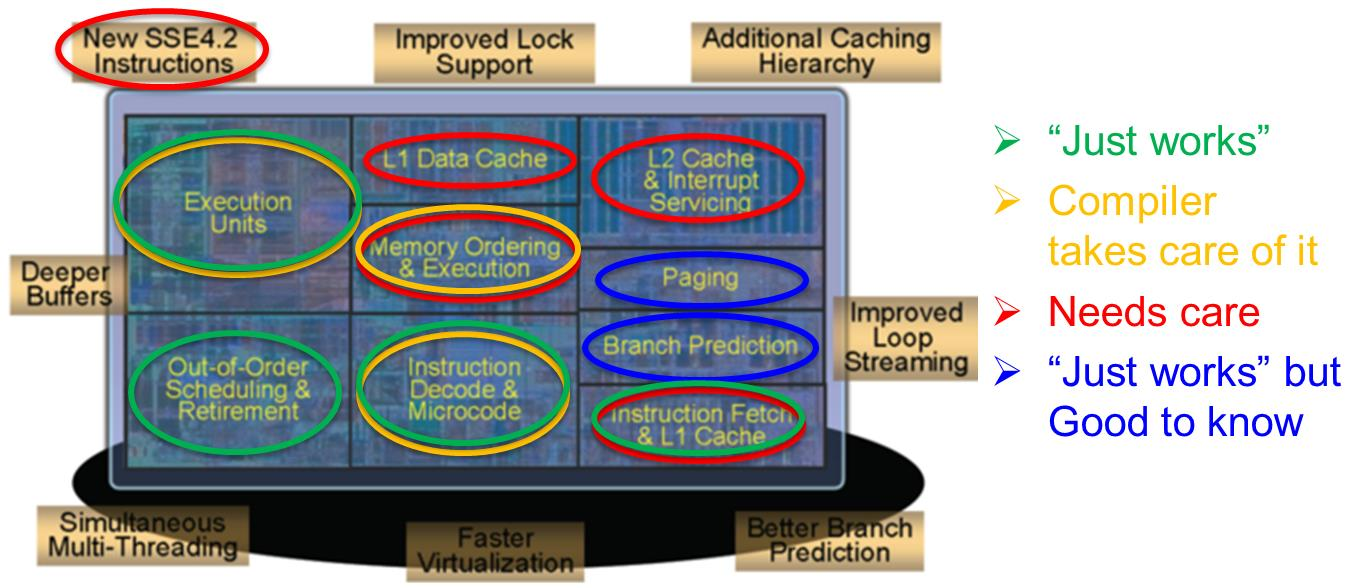
\includegraphics[width=0.9\textwidth]{content/1/chapter3/images/1.jpg}\\
圖3.1 - Pentium CPU的模具圖像,帶有功能區標記(來源:Intel)
\end{center}

圖像頂部是主要功能區域。如果是第一次看到這樣的圖片,最令人吃驚的細節可能是執行單元,也就是做加法、乘法和我們認為是CPU主要功能的部分,實際上甚至不佔用四分之一的硅面。剩下的是其他的東西,其目的基本上是使加法和乘法能夠有效地工作。並且,處理器有許多具有不同功能的組件。這些組件有一些是獨立工作的,開發者無需做什麼就可以使用它們。有些需要精心安排機器碼,這主要由編譯器完成。但是,超過一半的硅面用於組件,這些組件不僅僅是進行優化,還為了獲得處理器的最大性能。開發者需要了解它們是如何工作的,它們可以做什麼和不可以做什麼,以及什麼會影響它們的操作效率(積極和消極)。如果需要真正出色的性能,即使使用那些運行良好的部分,也可以從這些組件中受益。

有很多關於處理器架構的書,包括設計師用來提高性能的所使用的硬件技術。這些書可以作為知識的來源,但本書不會再成為這樣的書。這裡,我們將著重於探索發揮硬件性能的實際方法,我們先從CPU開始。













































